\documentclass[tikz,border=2pt]{standalone}
\usepackage{amsmath,amssymb}
\usepackage{tikz}
\usetikzlibrary{arrows.meta}

\begin{document}
% Moving along a curve gamma(t) through the level sets of f: the rate of change of f along
% the curve is the dot product of the gradient with the velocity vector.
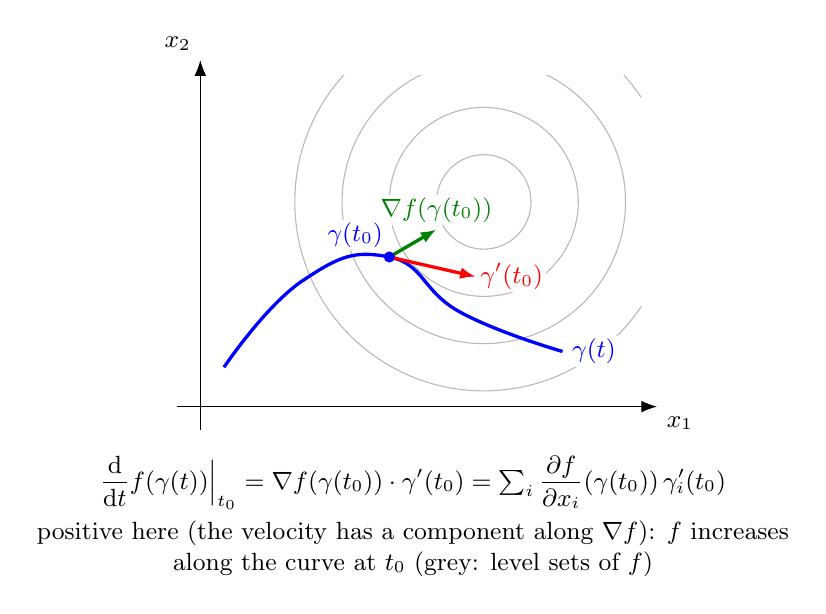
\begin{tikzpicture}[every node/.style={font=\small}, >={Latex[length=2mm]}, lab/.style={font=\small, fill=white, inner sep=1pt}]
	\begin{scope}
		\clip (0,0) rectangle (5.6,4.2);
		\foreach \r in {0.6,1.2,1.8,2.4} {\draw[gray!55] (3.6,2.6) circle (\r);}
	\end{scope}
	\fill[gray] (3.6,2.6) circle (1.5pt);
	\draw[->] (-0.3,0) -- (5.8,0) node[below right] {$x_1$};
	\draw[->] (0,-0.3) -- (0,4.4) node[above left] {$x_2$};
	\draw[blue, very thick] plot[smooth, tension=0.8] coordinates {(0.3,0.5) (1.3,1.6) (2.4,1.9) (3.3,1.2) (4.6,0.7)};
	\node[blue, anchor=west, lab] at (4.68,0.7) {$\gamma(t)$};
	\coordinate (P) at (2.4,1.9);
	\draw[->, red, very thick] (P) -- (3.5,1.65) node[right, lab] {$\gamma'(t_0)$};
	\draw[->, green!50!black, very thick] (P) -- (3.0,2.25) node[above, lab, yshift=1pt] {$\nabla f(\gamma(t_0))$};
	\fill[blue] (P) circle (2pt);
	\node[blue, anchor=south east, lab] at (2.36,1.98) {$\gamma(t_0)$};
	\node[anchor=north, align=center] at (2.7,-0.5) {$\dfrac{\mathrm{d}}{\mathrm dt}f(\gamma(t))\Big|_{t_0}=\nabla f(\gamma(t_0))\cdot\gamma'(t_0)=\sum_i\dfrac{\partial f}{\partial x_i}(\gamma(t_0))\,\gamma_i'(t_0)$\\[3pt] positive here (the velocity has a component along $\nabla f$): $f$ increases\\ along the curve at $t_0$ (grey: level sets of $f$)};
\end{tikzpicture}
\end{document}
